\chapter{Tools} 
Multiple tools were used in the process of creating the demo application for
this paper including the Unity game engine, Blender as a modeling and animation
software, and MakeHuman as a model creation tool. This chapter discusses the
built-in functionalities which make the mentioned tools an effective choice.

\section{MakeHuman}
MakeHuman is an open source tool for making 3D characters. It provides
a convenient way of acquiring a human model which is customizable and can be
exported in various formats in order to be used in other software programs. The
key factors which make this tool suitable for use in the demo application are the
options it provides regarding the complexity of the topology of the model's
mesh, and the choice of skeleton rig. One of the rig presets, which is shown in
Fig. \ref{fig:mh_rig}, is specifically designed to be used for video games. Many
additional cosmetic choices are also offered by the program, allowing for a full
customization of the character. The model is automatically rigged and ready to
be exported and used in an animation software. 

\begin{figure}[!h]
    \centering
    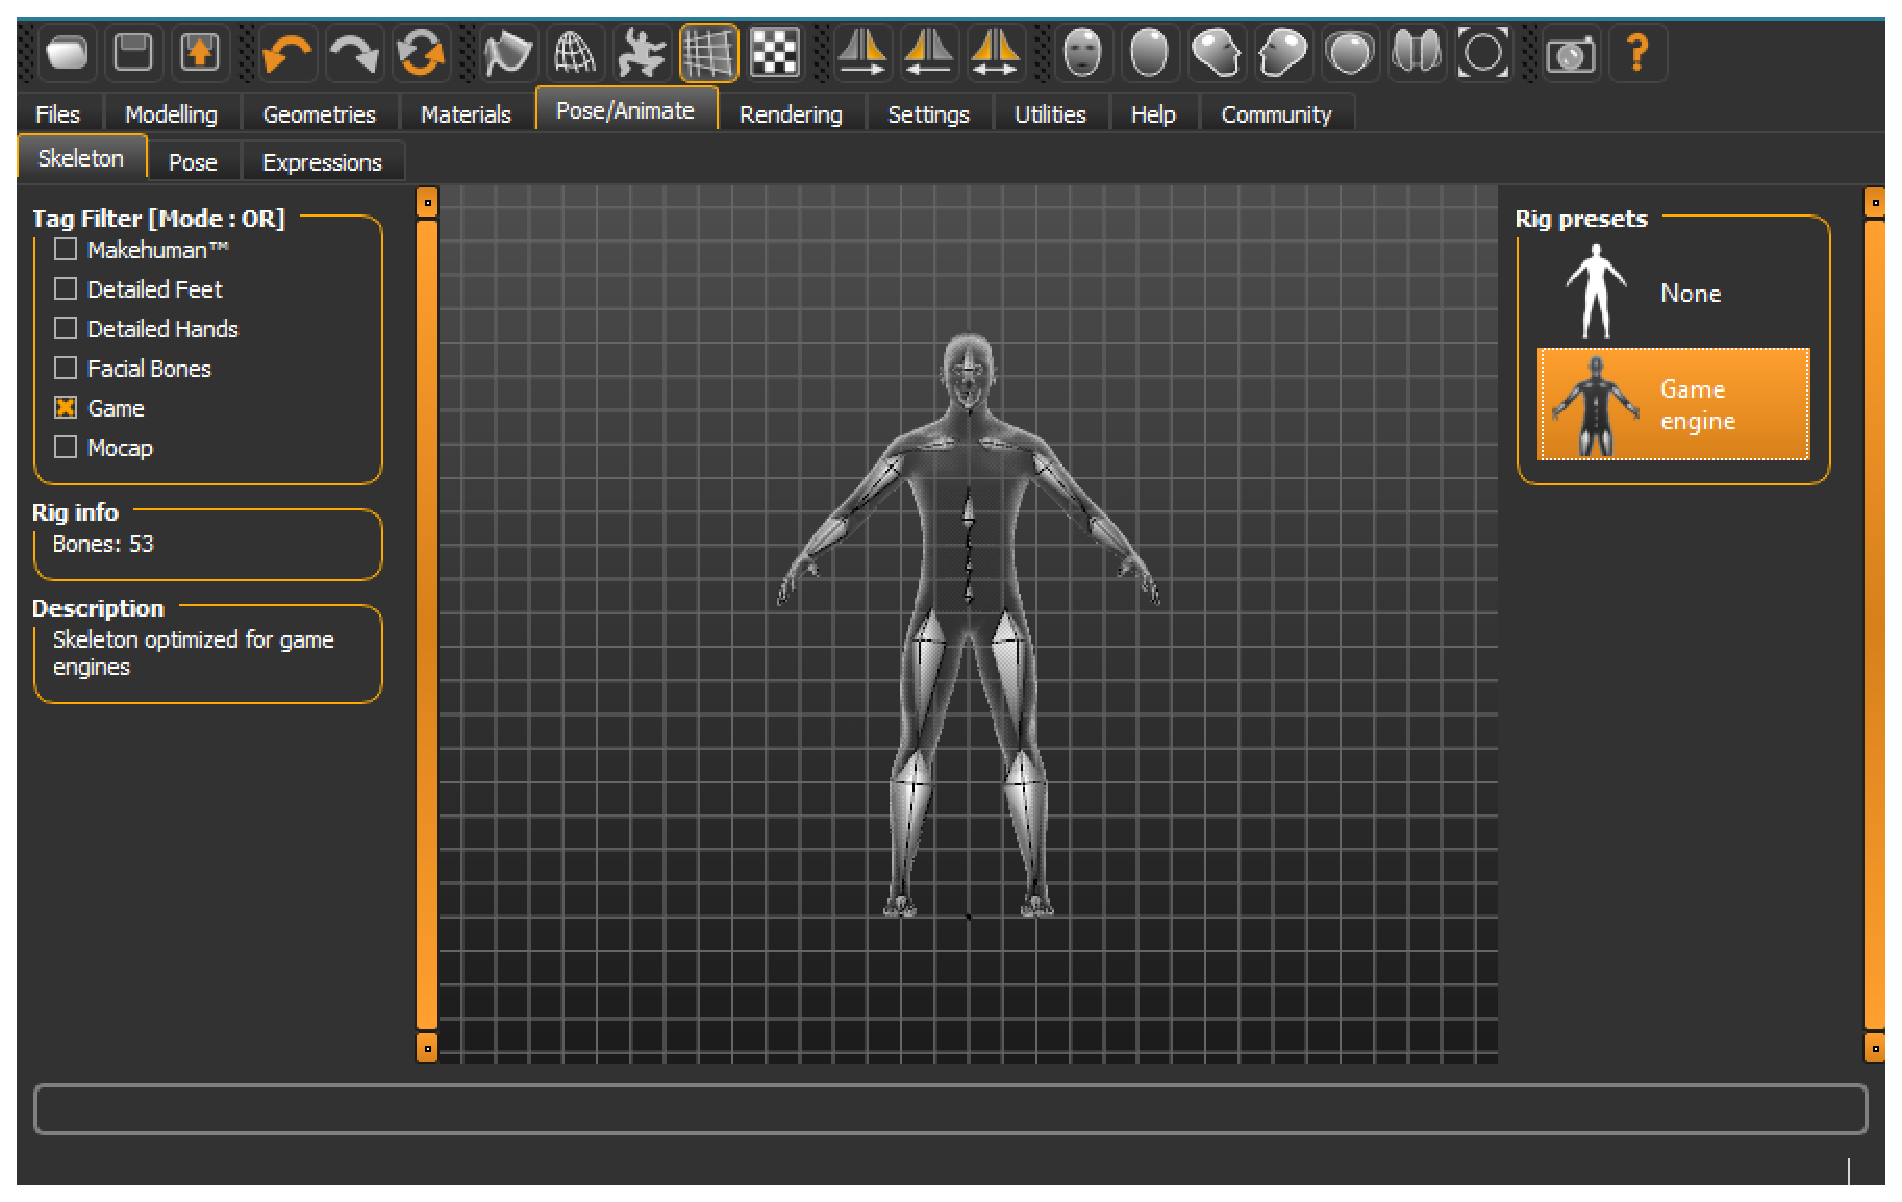
\includegraphics[width=0.9\textwidth]{grafika/make_human_rig.eps}
    \caption{MakeHuman rig selection}
    \label{fig:mh_rig}
\end{figure}

\section{Blender}
The tool for modeling and animation used for the demo application is
Blender. It is a free and open source tool offering a suite of functionalities
including the creation of 3D models, rigging, and animation. 

% The program enables
% users to import models in various formats, which allows the user to use
% externally generated models, such as the ones created in MakeHuman, and animate
% them. 

Blender offers the functionality of importing existing models in various formats
including the \textit{collada} format \cite{collada} which is the default export
option in MakeHuman. Models can also be created from scratch. Blender offers
a 3D modelling tool to create a desired mesh. A custom rig can also be
constructed and attached to the created model. Weights can be painted on the
mesh's vertices for each bone in order to define how much the position of each vertex
depends on the given bone position. 

\begin{figure}[!h]
    \centering
    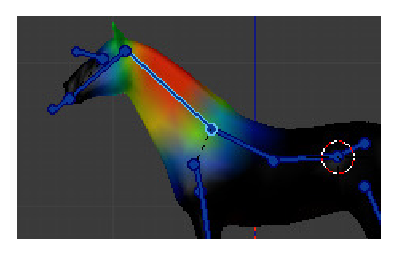
\includegraphics[width=0.4\textwidth]{grafika/weight_paint.eps}
    \caption{Weight painting in blender. Source: \cite{unity_weights}}
    \label{fig:weights}
\end{figure}

Lastly, an animation sequence can be created for an existing mesh and rig using
the character animation pose editor. The user can define poses for different
points in time by creating key frames on a timeline, and blender interpolates the
bone positions in between the key frames. This is used to create baked animations
for characters and objects, as well as defining animations that are later
blended with IK procedural animations. An animated model can be exported in the
\textit{fbx} format to be used in other software programs. Unity also supports
importing a model from a \textit{.blend} file which is the extension of
a blender project file. 


\section{Unity}
The Unity game engine is the one tool which was non-negotiable as this work
is meant to specifically focus on the usage of inverse kinematics in said game
engine. Nevertheless, it is a good selection for this use case due to its
advanced 3D support, the built-in packages and functionalities which help
with implementing the techniques discussed in this work, and the overall popularity of
the engine and large community built around it which results in a substantial
amount of documentation and support. 

\subsection{Importing Animations}
Unity enables users to import animated models from external sources using an
\textit{fbx} file or by importing project files from 3D modeling and animation
software such as Blender, Autodesk Maya, Cinema4D, or Autodesk 3ds Max
\cite{unity_import}. However, the modeling software must be installed on the
user's machine in order to import a model from project files, as Unity uses the
programs themselves to unpack the file. 

When importing an animated model into Unity, the import settings allow the user
to break the animation into multiple parts based on start and end times as
demonstrated in Fig. \ref{fig:anim_chunk}. This is convenient, as it allows
multiple animations made in Blender to be placed on a timeline one after the
other as a single animation, which can then be broken up in Unity. It also
allows the user to extract multiple different variations of the same animation,
such as importing the full animation as one whole chunk and also breaking it up
into separate animations for different use cases.

\begin{figure}
    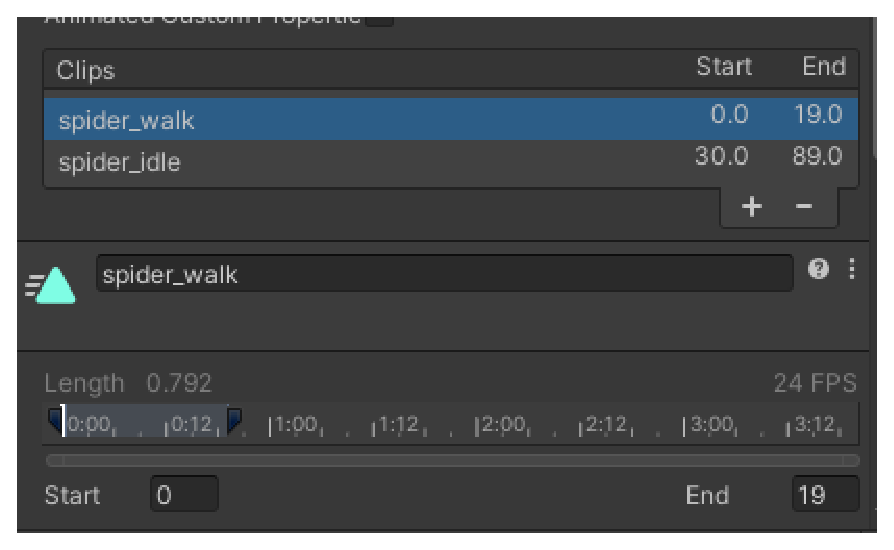
\includegraphics[width=0.5\textwidth]{grafika/animation_chunk_1.eps}
    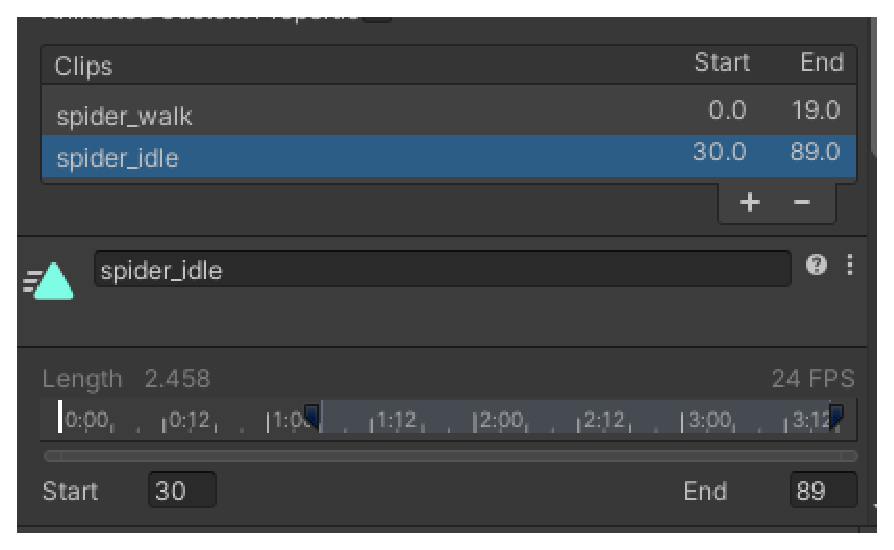
\includegraphics[width=0.5\textwidth]{grafika/animation_chunk_2.eps}
    \caption{Animation clips extracted from a single animation during import}
    \label{fig:anim_chunk}
\end{figure}

\subsection{Animator Controller}
An \textit{Animator controller} allows the user to maintain a set of animation
clips, and the associated transitions which control the flow between each clip
in the form of a state machine as shown in Fig. \ref{fig:anim_state}. Animations must be
added to an \textit{Animator controller} in order to be used by a Unity
\textit{GameObject} \cite{unity_animator}. States can also be controlled
procedurally from scripts by accessing an \textit{Animator} component which must
be attached to the Unity \textit{GameObject} and must hold a reference to the
given \textit{Animator controller}.
 
\begin{figure}
    \centering
    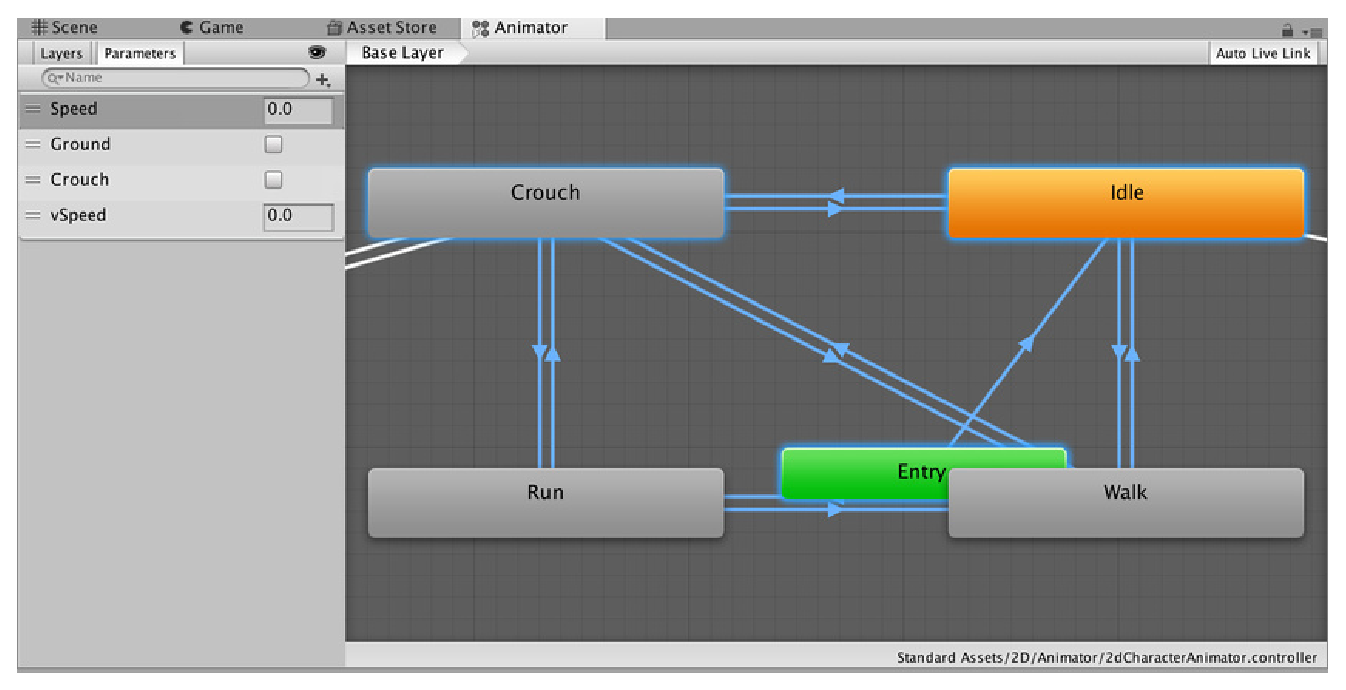
\includegraphics[width=\textwidth]{grafika/animator_controller.eps}
    \caption{Animator controller animation state machine \cite{unity_animator}}
    \label{fig:anim_state}
\end{figure}

The \textit{Animator controller} also has built in IK functionality. This is only
available for humanoid models which have a correctly configured avatar
\cite{unity_ik}. A humanoid avatar is available for models which adhere to a set
of defined general guidelines. In essence, a model which falls into the humanoid
category must have at least 15 bones which are organized in a way which
resembles a human skeleton \cite{unity_humanoid_import}. Humanoid characters
have a few additional functionalities. Namely, because of the criteria required
to qualify as a humanoid model, these models are all similar in structure and as
such, animations can be mapped from one humanoid model to another
\cite{unity_humanoid_avatars}. Additionally, these model's have built in
functionality which allows the developer to procedurally control the models IK
weights and positions using the \textit{SetIKPositionWeight,
SetIKRotationWeight, SetIKPosition, SetIKRotation, SetLookAtPosition,
bodyPosition, bodyRotation} functions \cite{unity_ik, unity_humanoid_avatars}.
Because these methods are not available to skeletal structures which do not fit
the humanoid description, they are not applicable to the demo application
created for this paper.

\subsection{Animation Rigging Package}

The Animation Rigging package is available in the Unity Package Manager, and it
provides a much more general approach to the application of inverse kinematics
to skeletal animations. After setting up a rig for a model with an Animator
component, a mix of predefined constraints can be added to enhance the rig,
which are briefly described in Table \ref{tbl:ar_constraints}. The main
constraint of interest for this paper is the \textit{Chain IK Constraint} which
implements the FABRIK algorithm. This constraint was useful in creating a proof
of concept for the spider before creating the FABRIK script. It also provided
a good basis for the public interface which such a script should have to
function well in the Unity environment.

\begin{table}
    \centering
    \begin{tabular} { |m{5cm}|m{10cm}| }
        \hline
        Blend Constraint & \footnotesize Allows the constrained object to blend
        between the position and rotation of two other objects. \\
        \hline
        Chain IK Constraint & \footnotesize Applies IK to a hierarchy of objects
        defined by a root and tip. Implements the FABRIK solver. \\
        \hline
        Damped Transform & \footnotesize Damps the position and rotation
        transform values from the source object to the constrained object in
        a hierarchy, increasing in time delay for each next object. \\
        \hline
        Multi-Aim Constraint & \footnotesize Rotates an object to face a chosen
        source object. Can have more than one source object with defined
        weighting. \\
        \hline
        Multi-Parent Constraint & \footnotesize Moves and rotates an object as
        if it is the child of another object in the hierarchy. Does not affect
        scale, and it can have more than one source object with defined
        weighting. \\
        \hline
        Multi-Position Constraint & \footnotesize Moves an object to follow
        a source object. Can have more than one source object with defined
        weighting. \\
        \hline
        Multi-Referential Constraint & \footnotesize Allows an object to act as
        the parent to multiple referenced objects.\\
        \hline
        Multi-Rotation Constraint & \footnotesize Rotates an object to match the
        rotation of its source object. Can have more than one source object with
        defined weighting. \\
        \hline
        Override Transform & \footnotesize Allows a constrained object's
        position and rotation to be overridden in world space, local space, or
        pivot space, by the displacement of the override transform, or by
        precise numerical values. \\
        \hline
        Twist Chain Constraint & \footnotesize Allows controlling world
        rotations on both ends of an object chain hierarchy. The two rotations
        are interpolated along the chain to create a smooth animated hierarchy.
        \\
        \hline
        Twist Correction & \footnotesize Applies a defined percentage of the
        rotation of a source object to chosen twist node objects. \\
        \hline
        Two Bone IK Constraint & \footnotesize Applies IK to a hierarchy
        composed of 2 bones which allows the use of a one target and one hint
        object for control. \\
        \hline

    \end{tabular}
    \caption{An available set of predefined constraints from the Animation
    Rigging package which can be applied to a rig
\cite{unity_animation_rigging}.}
    \label{tbl:ar_constraints}
\end{table}
